\chapter{The case of WASP-77Ab}\label{chap:wasp77}

\section{The system}
The third exoplanet we followed-up in this work, WASP-77Ab, was first presented by \cite{Maxted2013}. WASP-77Ab has a mass of $1.8\,{\rm M_{Jupiter}}$ and a radius of $1.2\,{\rm R_{Jupiter}}$, and orbital period of 1.36 days. It transits a G8 star in the visual binary system with a separation of 3.3 arcsec.

\section{Transit Parameters and Physical Properties}
Table~\ref{tab:wasp77} lists the results of the global fit of WASP-77Ab, in comparison with the values from its discovery paper \citep{Maxted2013} on which photometry and RV data were used. No other previous work has reported bulk measurements for this system.

Almost all the stellar parameters are in agreement with \citep{Maxted2013}, except for a $-9.7\sigma$ difference in the stellar surface gravity $\log{g}$, where our reported value is preciser.  

The primary transit parameters, as well as the RV parameters and the derived planetary parameters, are consistent with the results from \cite{Maxted2013}.


\begin{landscape}
\begin{longtable}{llcc}
\caption{System parameter of WASP-77A}
\label{tab:wasp77}
\centering
\tabularnewline
\hline 
~~~~~Parameter & Units & This work & \cite{Maxted2013}\\
\hline
\smallskip\\\multicolumn{2}{l}{Stellar Parameters:}&\smallskip\\
~~~~$M_*$\dotfill &Mass (\(M_\odot\))\dotfill &$0.903^{+0.066}_{-0.059}$ & $1.002\pm0.045$\\
~~~~$R_*$\dotfill &Radius (\(R_\odot\))\dotfill &$0.910^{+0.025}_{-0.023}$ & $0.955\pm0.015$\\
~~~~$L_*$\dotfill &Luminosity (\(L_\odot\))\dotfill &$0.743^{+0.065}_{-0.058}$ & \\
~~~~$\rho_*$\dotfill &Density (cgs)\dotfill &$1.692^{+0.056}_{-0.069}$\footnote{a} & $1.629^{+0.023}_{-0.028}$\footnote{a}\\
~~~~$\log{g}$\dotfill &Surface gravity (cgs)\dotfill &$4.476^{+0.014}_{-0.015}$ & $4.33\pm0.08$\\
~~~~$T_{\rm eff}$\dotfill &Effective Temperature (K)\dotfill &$5617\pm72$ & $5500\pm80$\\
~~~~$[{\rm Fe/H}]$\dotfill &Metallicity \dotfill &$-0.10^{+0.10}_{-0.11}$ & $0.00\pm0.11$\\
~~~~$Age$\dotfill &Age (Gyr)\dotfill &$6.2^{+4.0}_{-3.5}$ & $0.5-1.0$\\

\smallskip\\\multicolumn{2}{l}{Planetary Parameters:}&\smallskip\\
~~~~$R_P$\dotfill &Radius (\rj)\dotfill &$1.183^{+0.034}_{-0.031}$ & $1.21\pm0.02$\\
~~~~$M_P$\dotfill &Mass (\mj)\dotfill &$1.650^{+0.082}_{-0.075}$ & $1.76\pm0.06$\\
~~~~$P$\dotfill &Period (days)\dotfill &$1.3600290^{+(18)}_{-(20)}$ & $1.3600309\pm(20)$\\
~~~~$e$\dotfill &Eccentricity \dotfill&$0.0074^{+0.0075}_{-0.0051}$\\
~~~~$a$\dotfill &Semi-major axis (AU)\dotfill &$0.02323^{+0.00056}_{-0.00052}$ & $0.0240\pm0.00036$\\
~~~~$\omega_*$\dotfill &Argument of Periastron (Degrees)\dotfill &$-30^{+170}_{-120}$\\
~~~~$\rho_P$\dotfill &Density (cgs)\dotfill &$1.240^{+0.060}_{-0.067}$ & $1.33\pm0.04$\footnote{b}\\
~~~~$logg_P$\dotfill &Surface gravity \dotfill &$3.467^{+0.012}_{-0.015}$ & $3.441\pm0.008$\\
~~~~$T_{eq}$\dotfill &Equilibrium temperature (K)\dotfill &$1695^{+25}_{-24}$\\
~~~~$\Theta$\dotfill &Safronov Number \dotfill &$0.0717\pm0.0021$\\
~~~~$\fave$\dotfill &Incident Flux (\fluxcgs)\dotfill &$1.87^{+0.11}_{-0.10}$\\

\smallskip\\\multicolumn{2}{l}{Primary Transit Parameters:}&\smallskip\\
~~~~$T_0$\dotfill &Transit Time (\bjdtdb)\dotfill &$2457420.88439^{(+80)}_{(-85)}$ & $2455870.44977\pm(20)$\\
~~~~$i$\dotfill &Inclination (Degrees)\dotfill &$88.91^{+0.74}_{-0.95}$ & $89.4^{+0.4}_{-0.7}$\\
~~~~$R_P/R_*$\dotfill &Radius of planet in stellar radii \dotfill &$0.13352^{+0.00074}_{-0.00070}$\\
~~~~$a/R_*$\dotfill &Semi-major axis in stellar radii \dotfill &$5.493^{+0.060}_{-0.075}$\\
~~~~$b$\dotfill &Impact parameter \dotfill &$0.105^{+0.089}_{-0.071}$ & $0.06^{+0.07}_{-0.05}$\\
~~~~$\delta$\dotfill &Transit depth (fraction)\dotfill &$0.01783^{+0.00020}_{-0.00019}$\\
~~~~$u_{1,B}$\dotfill &linear LD coeff., B band \dotfill &$0.680\pm0.054$&\\
~~~~$u_{2,B}$\dotfill &quadratic LD coeff., B band\dotfill &$0.140^{+0.052}_{-0.053}$&\\
~~~~$u_{1,clear}$\dotfill &linear LD coeff., \emph{clear} band \dotfill &$0.386\pm0.029$\\
~~~~$u_{2,clear}$\dotfill &quadratic LD coeff., \emph{clear} band \dotfill &$0.227\pm0.029$&\\
~~~~$u_{1,I}$\dotfill &linear LD coeff., I band \dotfill &$0.311\pm0.025$&\\
~~~~$u_{2,I}$\dotfill &quadratic LD coeff., I band \dotfill &$0.294\pm0.033$&\\
~~~~$u_{1,R}$\dotfill &linear LD coeff., R band \dotfill &$0.312\pm0.023$\\
~~~~$u_{2,R}$\dotfill &quadratic LD coeff., R band \dotfill &$0.237^{+0.029}_{-0.028}$\\
~~~~$T_{14}$\dotfill &Total transit duration (days)\dotfill &$0.08952^{+0.00053}_{-0.00051}$\\
~~~~$P_T$\dotfill &A priori non-grazing transit prob \dotfill &$0.1578^{+0.0029}_{-0.0025}$\\
~~~~$P_{T,G}$\dotfill &A priori transit prob \dotfill &$0.2064^{+0.0039}_{-0.0033}$\\
~~~~$\tau$\dotfill &Ingress/egress transit duration (days)\dotfill &$0.01075^{+0.00032}_{-0.00015}$\\

\smallskip\\\multicolumn{2}{l}{RV Parameters:}&\smallskip\\
~~~~$e\cos{\omega_*}$\dotfill & \dotfill &$-0.0033^{+0.0041}_{-0.0065}$\\
~~~~$e\sin{\omega_*}$\dotfill & \dotfill &$-0.0002^{+0.0061}_{-0.0073}$\\
~~~~$K$\dotfill &RV semi-amplitude (m/s)\dotfill &$323.4^{+3.7}_{-3.3}$ & $321.9\pm3.9$\\
~~~~$M_P\sin i$\dotfill &Minimum mass (\mj)\dotfill &$1.649^{+0.082}_{-0.075}$\\

\smallskip\\\multicolumn{2}{l}{Secondary Eclipse Parameters:}&\smallskip\\
~~~~$T_S$\dotfill &Time of eclipse (\bjdtdb)\dotfill &$2457659.5665^{+0.0038}_{-0.0056}$\\
~~~~$b_S$\dotfill &Eclipse impact parameter \dotfill &$0.104^{+0.089}_{-0.071}$\\
~~~~$\tau_S$\dotfill &Ingress/egress eclipse duration (days)\dotfill &$0.01076^{+0.00035}_{-0.00023}$\\
~~~~$T_{S,14}$\dotfill &Total eclipse duration (days)\dotfill &$0.0895^{+0.0013}_{-0.0014}$\\
~~~~$P_S$\dotfill &A priori non-grazing eclipse prob \dotfill &$0.1578^{+0.0018}_{-0.0012}$\\
~~~~$P_{S,G}$\dotfill &A priori eclipse prob \dotfill &$0.2063^{+0.0025}_{-0.0016}$\\
\hline
%\end{tabular}
%\tablefoot{
%\tablefoottext{a}{Value converted to cgs units multiplying by the Sun density $\rho_{\odot}=1.408\,$cgs.}
%\tablefoottext{b}{Value converted to cgs units multiplying by the Jupiter density $\rho_{J}=1.33\,$cgs.}
%\tablefoottext{c}{Values enclosed in parentheses correspond to the uncertainties of the last digits of the nominal value.}
%}
\end{longtable}
\end{landscape}

\section{Transit Timing Variations}

As in the previous targets, we computed a refined linear ephemeris equation for WASP-77A considering 11 transit times:
\begin{equation} \label{eq1_w77}
T_{\rm C}(E)=2457420.88439\pm(85)+E \cdot 1.36002854\pm(52)
\end{equation}

In Table~\ref{tab:wasp77} are listed the TTV values of our transit times and from previous works \citep{Turner2016,Maxted2013} of WASP-77Ab and, at the bottom of Figure XXX are plotted versus epoch. The scatter of all the transit times is about $RMS=121$ seconds. 

The epochs $175$ and $229$ are above $2\,\sigma$ from the expected transit time following the linear ephemeris, while all the others epochs lie within $1.5\,\sigma$ from it. When removing the epochs $175$ and $229$, the RMS decreases to 88 seconds. 

Considering all the transit times, the linear fit has $\chi^{2}_{red}=1.4$, and the second degree polynomial has $\chi^{2}_{red}=1.39$ . However, we chose the linear fit as it suppose a simpler model.

\begin{table}
\caption{Transit mid-times for WASP-77Ab}
\label{times_wasp77}
\centering
\begin{tabular}{cccc}
\hline \hline
Epoch & Transit mid-time & TTV & References\\
      & (${\rm BJD_{TDB}}$) & (min) &  \\
\hline
-1140 & $2455870.45054$ & $-2.0\pm1.5$ & 1 \\
-845 & $2456271.65888$ & $-2.0\pm1.4$ & 2 \\
-659 & $2456524.62617$ & $0.8\pm1.8$ & This work\footnote{a} \\
-606 & $2456596.70591$ & $-1.7\pm1.5$  & This work\footnote{a}  \\
-92 & $2457295.7626$  & $1.2\pm1.3$& This work \\
-89 & $2457299.84119$ &  $-1.0\pm1.3$ & This work \\
175 & $2457658.88744$ & $-2.8\pm1.5$ & This work\\
177 & $2457661.60987$   & $0.6\pm1.7$ & This work\footnote{a} \\
183 & $2457669.77054$ &  $1.4\pm1.4$  & This work  \\
229 & $2457732.33382$ & $4.2\pm1.4$& This work\footnote{a} \\
447 & $2458028.8159$  & $-1.8\pm6.5$ & This work\\ 
\hline
\end{tabular}
%\tablebib{(1) \citet{Maxted2013}; (2) \cite{Turner2016}.}
%\tablefoot{
%\tablefoottext{a}{From the Exoplanet Transit Database (ETD)  \url{var2.astro.cz/ETD}}}
\end{table}

\section{Limits on an additional perturber}
For the WASP-77Ab system the results are somewhat similar to WASP-19b. We refer to Fig.~\ref{megno_wasp77}. The measured RMS of mid-transit timing variations around the linear ephemeris was $\rm TTV_{\rm RMS}=121\rm s$. For interior mean-motion resonances the 1:2 and 2:3 commensurabilities could cause the observed $\rm TTV_{\rm RMS}$ by an additional planet of mass around $3.5~M_{\oplus}$ and $7~M_{\oplus}$. However, the 2:3 resonance is very close to the general instability area rendering the orbit likely to be unstable. Further a $1~M_{\oplus}$ mass planet at the 1:3 interior resonance could also cause a $\rm TTV_{\rm RMS}$ of 121 s. A $2~M_{\oplus}$ mass planet located at the 3:5 resonance, although relatively close to the inner edge of the general instability region, could also explain the observed timing variation. For exterior 
mean-motion resonances of 2:1, 3:1 and 4:1 an additional planet of mass $3.5~M_{\oplus}, 4.5~M_{\oplus}$ and $60~M_{\oplus}$, could cause a $\rm TTV_{\rm RMS}=121\rm s$, respectively. A subtle difference from the WASP-19b system is found at the 5:2 resonance, which does not exhibit any significant decrease in upper mass planet detection sensitivity.

\begin{figure}
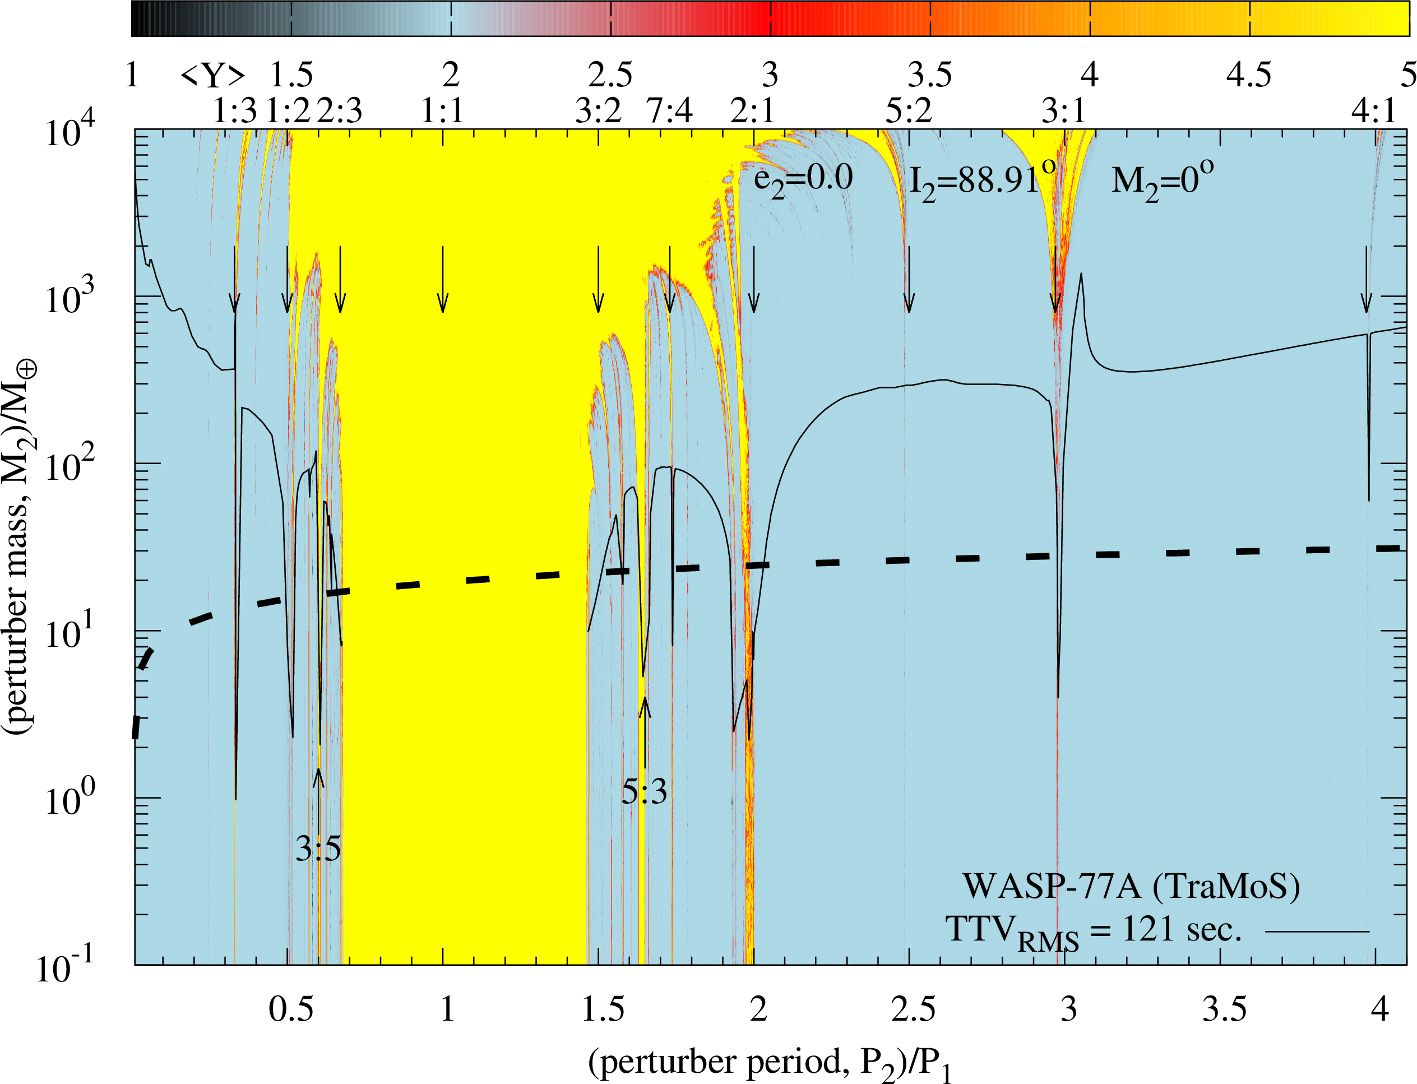
\includegraphics[width=1.0\columnwidth]{imagenes/WASP77_TraMos_121sec_Map001_GIMP_scaled.png}
\caption{Same as Fig.~\ref{megno_wasp18}, but this time for WASP-77 with an $\rm TTV_{\rm RMS}$ of 121 s. The RMS for the radial-velocity measurements was $(12.0\,\rm m/s)$.
\emph{See electronic version for colors}.}
\label{megno_wasp77}
\end{figure}